\section{Previous Approaches to Dispatching}

% \fcomment{I need to rework this as it is not really a state
%   of the art in the current form ... we also need to present that fact
%   that not that much people do consider postponement of actions
%   ... except maybe for dynamic controllability problem ... this may be
%   the key for this part. WE can present proactive approaches as being
%   the general agreement except for the special case of dynamic
%   controllability where 3DC+  introduces wait actions which in fact put
%   time-points that need to be deferred. We on the other hand try to
%   look at another aspect that may trigger the decision to defer an
%   actions based on its purpose}

Dealing with plan execution is not a new problem and we can find a lot
of work that relates to this during the last decades. Still, it is
pretty rare to see work that envisage that actions could be
postponed except when this is necessary to not break the current
plan. 


The most prominent work is related to the dispatchability of simple 
temporal networks (STN) \cite{mus98a}. The core of the problem is to
ensure that the temporal constraints can be propagated efficiently
within the plan in order to allow the executive to decide quickly
whether an action should be started or not while ensuring the plan
consistency. In order to accomplish such a task, the STN supporting
the plan to be dispatched is transformed into a All-Pairs network and
stripped of unnecessary edges, resulting often on a more compact
temporal network and lessen the propagation cost of its updates. The
role of the executive is to select time-points within the current
execution bounds and propagate its value within the simplified
network. Still, while this work contribute to ensure that execution
time are correctly propagated within the plan with a limited cost, it
does not directly address how to decide what value should be set for a
given time-point in the scope of its possible values. More specifically
it is still the role of the executive to decide whether it should
start an action as early as possible or consider it as not urgent. 

When dealing with least-commitment planning solution this decision is
deferred to the plan executive. For example in \cite{mus98c}, the 
executive is defined as having two responsibilities: the selection and scheduling of plan
events for execution. The executive needs to
be highly reactive as it is necessary to function in a real-time
environment. One solution offered for dispatching events efficiently
is the proactive approach. This approach greatly reduces the plan
flexibility, and therefore robustness, as all start time-points are
grounded to a specific value which is compatible with the initial
constraints. In order to avoid having a procrastinating system the
overall agreement in term of policy is to start an action as early as
possible (ref ?). 

% \fcomment{Therefore, one reoccurring problem of dispatchability is finding a way
% of balancing efficiency, proactive, with flexibility,deferred.}
\fcomment{We need to update this to reflect that it is not ETS}
%There have been many uses of these two approaches when dispatching plans, as
%previously shown, but a compromise to one is most often used rather than
%a balance. Demonstrated in the tool MAPGEN \cite{bresina03} which used
%the Earliest Time Solution (ETS) for generating and displaying plans
%very quickly. Then allowing the users to manipulate the plan afterwards,
%getting around the problem of ETS generating undesirable plans. What is
%needed is a way of using both proactive and deferred together giving a
%balanced approach to dispatching.

While in the general case it can be acceptable it
may become problematic when put in he context of potential new
objectives emerging during the mission.  Take our AUV example,
and apply the proactive approach globally -- assuming that all actions
can be completed on their minimum time.  As shown in 
Fig. \ref{fig:ex:proactive}, the proactive approach allows the
AUV to {\em Sample Vent2} before noon but as continue through
the plan it results in the AUV getting back to the {\em Surface}
by 12:21 and being stuck in the context of the current plan for the
next 7 hours and 39 minutes. Should the scientist want to {\em Sample Vent1}
the AUV will then be forced to re-plan accordingly and
go back and forth between the surface and the locations all other
again. By being blindly proactive, the AUV made its overall strategy
less efficient than if it took the option to procrastinate at {\em Vent2}
until it needs to get back to the surface. 


\begin{figure}
  \centering
  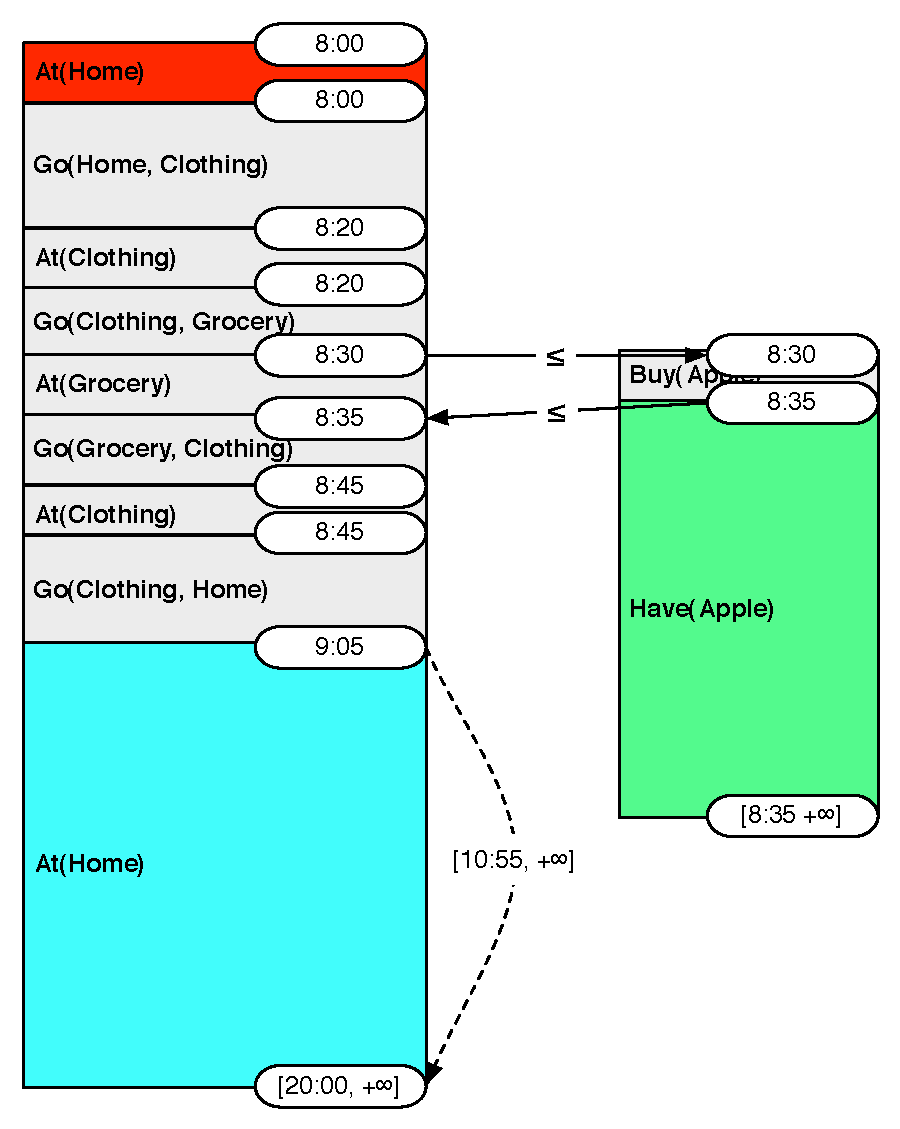
\includegraphics[width=0.8\columnwidth]{figs/example_early}
  \caption{proactive solution for the plan from Fig. \ref{fig:ex:plan}}
  \label{fig:ex:proactive}
\end{figure}

One case we have seen in literature where a time-point is
considered to be deferred is related to the dynamic controllability
issue with STNs with uncertainty (STNU). In \cite{morris01}, they propose 
an algorithm that during planning insert wait constraints within the
solution temporal network that will allow one time-point to wait until
an uncontrollable event occurs. In this case, the deterrence of the
execution of this time-point is enforced in order to ensure robust plan
execution despite exogenous uncontrollable events. In
\cite{gallien2006},  this approach is further discussed along with the
Makespan issue while dealing with least-commitment planners which can
insert unjustified waits within the plan potentially decreasing in turn the
overall performance of the system. Both of these approaches show that
when dealing with uncontrollable temporal constraints -- such as for
example the duration of a navigation task which depends on external
factors -- it is necessary to defer some actions in order to ensure
the plan execution. 

An alternative approach is related to wrok with soft constraints
within the temporal domain indicating preferences on actions timing
such as in \cite{khatib2001temporal}. This should provide  a general
solution for users to specify whether actions of the plan should be
preferably started. One problem with general frameworks dealing with
soft constraints though is their poor performances \cite{bartak2002}
as the general problem is NP-hard. Even though it can be reduced to a
more tractable (polynomial) solution by specifying preferences as
convex functions \cite{rossi2006learning}, the  
complexity is still at on the cubic in relation to the number of
variables. Moreover the solutions proposed do optimize the plan {\em
  a-priori} reducing then the plan flexibility which in turn make it
in  turn more prone to fail during execution.

Our work on the other hand is more complementary to previous work, indeed
while we do not really deal with dynamic controllability in our
problem -- which can anyway be treated as in this previous work -- the
core of our problem is not that much the observation of events during
execution (which is more a observation related impact) but instead we
are more focused on the knowledge that, within our agent, new
objectives can emerge at any time, and we want to avoid as much as
possible doing actions which are not ``urgent''. Similarly, while we do
not really deal with complex preferences specification that can help
improve the planned solution our purpose is to defer the decision to
start to execute actions within the plan to the executive allowing to
quickly adapt the plan without heavily relying on plan-repair or
re-planning solutions that could badly impact the system reactiveness.
By doing so, we take the risk of doing unnecessary actions as new
goals need to be integrated in the plan.

% s
% considered to be deferred is related to the approach proposed in 
% \cite{morris01} to deal with dynamic controllability issue. 
% \fcomment{following will be included in former para. Also we need to
%   address that it is in fact outside of our scope here ... we actually
% do not address dynamic controllability, worse we tend to make waiting
% actions more brittle in general as we take the upper bound  for needed
% actions}

% The only work where we see 

% % Dispatchability for a simple temporal network (STN) has been identified
% % with whether a plan is capable of fast execution, retains its
% % flexibility despite uncertainty in the plan, and all information is
% % available at execution \cite{mus98}.  To accomplish the task of
% % efficient execution, the STN's are transformed into All-Pairs networks
% % and striped of their unnecessary edges, which will often create a more
% % compact temporal network and esse the propagation of its updates.
% % The executive then selects a timepoint, within the bounds of the 
% % execution time, and every timepoint before it has
% % already been executed. It then sets the start time to the selected
% % timepoint and propagates the needed changes throughout the graph
% % \cite{mus98}. The process of selecting a timepoint can lead to
% % issues when two timepoints have the possibility of being executed at the
% % same time, where one should necessarily come first, but the incorrect
% % one gets selected first. This mistake can cause the STN to become
% % brittle, which leads to a higher chance of failure in the plan.

% % \fcomment{Need to continue to refine from here and talk about STNU and
% %   morris01 as  the only approach we know of where postponed events are present
% %   though the inserted wait}

% % Take our shopping example\fcomment{figure again}.  We'll say the agent wakes up
% % at 9 AM and the duration for traveling to the store is forty minutes
% % and buying the apples is ten minutes. Using the proactive approach, the
% % agent will start shopping as soon as possible and thus be done shopping
% % by 10 AM. The agent will then go directly home afterwards to satisfy the
% % ``home by 8 PM'' goal. However by doing so, the agent will be back
% % home by 11am with the constraint to stay at home for the next 9
% % hours. 
% % \fhighlight{If his wife} is then calling to ask him to buy extra things it will
% % results on hime to need to fully relax his current plan and go back
% % and forth between its home and the store all other again. By being
% % fully proactive the agent.\fcomment{Maybe what was meant initially
% % here is more related to dynamic controllability which mean that I need
% % to twek this text to be more related to a modelled
% % but uncontrolbale situation.}


% % However, the start time for this goal will be roughly
% % 11 AM, and if the agent wants to get some dessert before dinner it will
% % cause a failure in the plan. What this example shows is how EST can
% % severely reduce the flexibility of a mission. EST can also cause
% % inconsistency within the plan.

%  {\em \fhighlight{Therefore,} \cite{mus97}\fcomment{See comment before} added
% implied links between timepoints allowing the planner to find them
% efficiently.\fcomment{I don't get what you mean here}}


% Another issue with execution is uncertainty in the plan. The above
% example illustrates the uncertainty about when the agent should go home
% or if the agent will want to buy more food during the mission. A
% solution for execution uncertainty is the least-committed method, which
% waits until that last moment to execute events. This approach keeps the
% plans flexibility and it allows the executive to have all of the
% available information before making a choice (Block, 2006). However, it
% has been argued that the least-committed method is an inefficient
% solution because in a real-world environment an agent might idle for
% long periods of time (Gallien, 2006). This can severely decrease the
% overall performance of the system. Lets demonstrate the least-committed
% policy in our Shopping agent example using the same goals and durations
% as before. This time around the agent won't want to do anything until it
% is absolutely necessary to do it. The agent will then wait until 6:20 PM
% before leaving and will finish shopping at 7:20 PM this way the agent
% can be home by 8 PM. However, even though this keeps flexibility in the
% plan there are a few issues. If there happens to be traffic then the
% agent might not make it home by eight PM. Also the agent procrastinates
% all day just waiting to go shopping rather than starting early on in the
% day, which wastes valuable time. Their (Gallien, 2006) solution is to
% change the planning heuristic altering how their plan is created
% inevitably adjusting it for faster execution.


%%% Local Variables: 
%%% mode: latex
%%% TeX-master: "aaai13"
%%% End: 
